
\chapter{Tabligh, salafisme et djihadisme en France }
\textbf{Définitions, convergences et
divergences}


\mn{LUNDI 20 DECEMBRE 2021 (4e
cours)}

% --------------------------------------------------
\section{ Le courant tabligh : un piétisme qui prépare le terrain}
\label{sec:Tabligh}
Un rôle important pour la \emph{"reislamisation des communautés immigrés en France"}.

Né en 1927 au Pakistan, Mohammed Ilyas Kandhlawi. \paragraph{Les «jéhovah de l’islam» } avec l'idée du porte à porte pour leur apporter la "bonne nouvelle". Réputé apolitique, piétiste. Dans tous le sous-continent indien. Très implanté les communautés marocaines. 
\paragraph{En France}  «Foi et Pratique» (une dizaine de lieux de culte tout au plus), au départ représenté au CFCM, puis chaise vide. certains élus au CRCM, élu sous l'étiquette du RMF mais d'obédience tabligh. Cheikh Hammami, Wissam Tabbara comme principales figures.
Cette association a des biens à Grigny.
2008 : agression de journalistes de Canal+ en 2004 condamné.
Une approche orthodoxe et orthopraxe : Halal, prière (si on a raté la prière du vendredi, on sort de l'Islam). 


Dans les média, on a entendu parlé de ce mouvement par la polémique des voeux de bonne année de Maître Gims , converti par le mouvement Tabligh. 
\mn{Lire : \emph{La Barbe} de Omar Benlaala. idée de la captation par le charisme des prédicateurs. 1980-98
Gilles Kepel : \emph{Les Banlieues de l'islam
Naissance d'une religion en France}. Chapitre 43. Retrace l'arrivée de ce courant à Belleville. } 

\begin{Synthesis}
Ils sont peu nombreux aujourd'hui (10 centres de prière) au profit des salafistes, dont ils ont préparé le terrain.
\end{Synthesis}


% --------------------------------------------------
\section{Le courant salafiste : simple orthodoxie ou voie vers la radicalisation ?}

\subsection{Histoire et éléments généraux}

Issu de l'école Hanbaliste (9eme siècle), réputée la plus dure avec une rencontre du wahhabisme.

La typologie tripartite de Quitan Wicktorowicz (2006): "salafisme piétiste" (orienté vers la pratique, orthopraxi en direction des musulmans), «salafisme politique» (pacte de Najd avec les Saoud), « salafisme djihadiste » (celui de AlQaida mais aussi DAECH) (ensuite discutée, nuancée, complétée…). des causalités doctrinales qui légitiment la violence.
L'on trouve des concepts spécifiques à ce courant. Face à la « Jahiliya » contemporaine ou moderne (période pré-islamique ou état d'ignorance
de l'islam), les musulmans ont une obligation pour se mobiliser en vue
d’instaurer la notion de la souveraineté de Dieu, la « Hakimiya ». Un véritable État musulman est un état qui reconnaît l'autorité de Dieu en matière
légale. Pour lui, l’Etat qui abolit les lois de Dieu est un Etat tyrannique (de l'arabe "Taghout"
qui renvoie aussi bien à « tyran » qu'à « Idole »). \sn{\url{https://bibliotheques.wallonie.be/doc_num.php?explnum_id=5298}} 
\bi 
\item  La Jahiliya (l’ignorance pré-islamique) : il considère que les musulmans se sont éloignés
de l’islam, voire trahis. Il condamne, ainsi, la société égyptienne de son époque car elle
est tombée dans l’ignorance et la mécréance.
\item  Il appelle à construire « une génération avant-gardiste » qui a pour mission de rompre
les liens avec la société dite « corrompue », de changer le pouvoir politique et
d’imposer la Loi divine la chari’a afin que l’islam règne de nouveau Al hakimiya, la
souveraineté divine. Les pouvoirs politiques en terre d’islam et les musulmans qui
n’adhérent pas à leur idéologie sont considérés comme kouffâr (mécréants).
\item  Cette génération doit accomplir la « hijra », l’exil et la rupture pour se séparer des
sociétés qualifiées d’être impies.
\item  Le déclin des musulmans est dû d’abord à l’imitation des modèles idéologiques hors
de l’islam (le marxisme, l’impérialisme, etc.) Il considère que l’islam apporte la solution
complète à tous les sujets politiques, économiques, et sociaux. Il appelle à couper
court avec l’Occident en tant que civilisation qui a du mal à résoudre, d’abord, ses
 \item Le djihâd, dans son approche globale, est le moyen à utiliser pour conquérir le monde
impie « Kâfir». Il est devenu une obligation religieuse individuelle pour chaque
musulman contrairement à la définition classique de celui-ci comme devoir collectif
qui concerne q’une partie de la communauté des croyants.
\item Al wala wal bara (L’Alliance et le désaveu) \sn{\url{https://fr.scribd.com/document/80301054/L-Alliance-et-le-Desaveu-Al-Wala-wa-Al-Bara}} :Le terme takfir signifie littéralement « accusation d'athéisme » (kufr), et les takfiri sont ceux qui lancent cette accusation. Les takfiris considèrent les musulmans ne partageant pas leur point de vue comme étant des apostats, donc des cibles légitimes pour leurs attaques.
\ei



\subsection{En France}

Des transfuges du GSPC et du GIA en France pendant la décennie noire (Algérie) introduisent le salafisme dans la région lyonnaise à partir du milieu 90, puis Rhône-Alpes et Ile de France. Se combine avec la diffusion du hanbalo-wahhabisme (salafisme) via les livres, cassettes, puis DVD et internet à partir de la fin des années 90. Incubation salaf à Trappes, Strasbourg, Toulouse, 93, Marseille…
Environ 20 000 adeptes en France, surtout en Rhone Alpes, PACA et région parisienne. Grandes banlieues populaires des grandes villes. Pas plus d'une centaine de lieux salafistes.



-A propos d’une instance d’obédience hanbalo-wahhabite : la Ligue islamique mondiale (LIM) en France et en Europe (activités passées et ‘velléités de changement’?)

Ces mouvements salafistes, avec leur discours de rupture, ont visé à destabiliser les mosquées d'obédiance consulaire.


Quiétisme : impropre car par extrqmontin mais aspire à changer leq société

1745 : al wahhab, \textit{tawhid} unicité. Version pour enfant interdite
Maralih : en contexte musulman ne s’oppose pas à 

\paragraph{Différence entre Salafistes et Frères musulmans}
les frères musulmans sont prêts à discuter avec la société alors que les salafistes sont en retrait  (la société laique est \emph{Taghout} pour les salafistes).
Les Frères musulmans acceptent la mixité 
alors que les Salafistes non, même si on voit en Arabie Saoudite une évolution (cf Femme et permis de conduire). Droit des femmes : inflexion en Arabie saoudite


Eviter la notion de Frero-salafistes du fait des vraies différences.



\subsection{une idéologie rampante sans organisation centralisée}
\mn{Rapport montaigne : titre L'islam Salafiste : une idéologie rampante sans organisation centralisée}



\paragraph{Un fondamentalisme
contemporain}


Mouvement idéologique contemporain prônant le retour aux sources de
l'islam, le salafisme est complexe et son évolution constante. Les
salafistes veulent agir comme les pieux de la communauté musulmane
idéale des premiers temps, réunis autour du prophète de l'islam
Mohammed, érigé en modèle. Le salafisme constitue une tentative de
retrouver un islam « pur », tel celui pratiqué au temps du Prophète. En
ce sens, comme le souligne Mohamed-Ali Adraoui, le salafisme a à voir
avec \emph{« le mythe de l'âge d'or, celui du passé ou du paradis perdu
que l'on trouve dans de nombreuses sociétés, notamment lors des
situations de crise ou de bouleversements politiques majeurs. Les
sociétés se raccrochent à ce qu'elles peuvent pour supporter un présent
insupportable ou difficile. »} Le salafisme puise donc son dynamisme
dans les fractures qui divisent notre société mais aussi dans la crise
actuelle que traverse l'islam contemporain.

La dynamique salafiste est particulièrement complexe, parce qu'elle est
triple. Comme le note Mohamed Ali Adraoui, elle est à la fois
paradigmatique, méthodologique et orthopraxique :


\begin{itemize}
\item
  paradigmatique, car l'ensemble des actions entreprises, des
  comportements adoptés et des interprétations islamiques s'inscrivent
  en référence aux premières générations de croyants : le salafiste se
  distingue par la recherche systématique de l'imitation de Mahomet ;
\item
  méthodologique, car une norme n'est légitime que si elle est
  compatible avec la pratique des salafistes : ils condamnent et
  rejettent toute bid'a (innovation), qui caractérise les autres
  doctrines ;
\item
  
  orthopraxique, car le respect de ce cadre normatif religieux très
  strict garantit le salut du fidèle.
  
\end{itemize}


Aussi, le salafisme, s'il demeure un mouvement minoritaire au sein de
l'islam français et plus largement au sein de l'islam sunnite, est-il
particulièrement visible car ses adeptes, afin d'imiter les premiers
croyants musulmans et le Prophète Mahomet, adoptent tenues et
comportements de l'islam des premiers siècles ; port du \emph{qamis}
(longue tunique) pour les hommes et du \emph{niqab} (voile intégral)
pour les femmes. Les salafistes, en s'inscrivant dans la rupture --
aussi bien avec la société française qu'avec l'islam sunnite majoritaire
--, développent des pratiques de repli identitaire avant d'entamer la
\emph{hijra}, c'est-à-dire l'émigration dans une terre où l'islam est
majoritaire.

Le prosélytisme est particulièrement développé chez les salafistes. Le
salafisme quiétiste est prédicatif : il refuse la violence des
djihadistes et leur logique, mais prône au contraire l'attitude
missionnaire en vue de l'avènement d'un État et d'une société
islamiques.
\begin{quote}
    \emph{« Il s'agit bien d'insuffler aux musulmans une conscience
islamique par un retour à une pratique religieuse délivrée de tout ajout
postérieur à la révélation coranique et à l'apostolat prophétique. La
prédication permettra de créer un mouvement social aboutissant à une
nouvelle organisation du monde qui accordera à l'islam la
prééminence}\emph{. »}
\end{quote}
 L'éducation du fidèle et la prédication jouent
donc un rôle fondamental : le développement d'un discours moral et
orthodoxe, corrigeant constamment la croyance et les pratiques
religieuses, l'action dans les mosquées ou sur internet de prêcheurs
formés en Arabie Saoudite pour l'essentiel, et l'adoption d'un mode de
vie communautaire en sont les principaux vecteurs.

Mouvement ultra-conservateur, qui se nourrit du rejet de la modernité
politique, le salafisme -- de façon paradoxale -- est très moderne dans
son expression. La diffusion du salafisme s'appuie sur internet où se
constitue une véritable communauté salafiste virtuelle {[}voir 2.6.4{]},
relativement jeune et connectée. Il s'inscrit dans le cadre de la
mondialisation et alimente des dynamiques migratoires, qu'elles soient
temporaires, à l'instar des salafistes partant se former dans une
université islamique en Arabie Saoudite ou en Égypte, ou définitives
comme la hijra, l'émigration vers un pays musulman.



\paragraph{Public cible}


On estime à environ 15 000 à 20 000 le nombre de salafistes en France;
50 à 60 \% d'entre eux sont issus d'une famille d'origine maghrébine
tandis que 25 à 30 \% sont des convertis. Il s'agit d'une population
relativement jeune, entre la trentaine et la quarantaine.

Tous les musulmans ne sont pas également sensibles au salafisme :
l'attitude varie selon leurs caractéristiques ethno-nationales et leur
héritage culturel, ainsi que selon leur situation géographique et leur
culture politique. Ainsi constate-t-on que \textbf{les Maghrébins}
constituent un public cible du salafisme, car il s'immisce dans leur
fracture
identitaire et renvoie à \emph{« une image positive de l'arabité »} :
le salafisme apparaît donc comme un moyen de retrouver une identité
\emph{« perdue »} et de proposer une alternative à la seule identité
française perçue comme corruptrice. \textbf{Les Turcs,} en revanche, se
tournent relativement peu vers le salafisme, compte tenu de l'emprise
exercée sur les communautés turques par la DITIB et le Millî Görüş, qui
entretiennent un lien affectif et sentimental avec le pays d'origine et
rappellent régulièrement que le salafisme est un mouvement
essentiellement arabe, voire saoudien.

\textbf{Les convertis} représentent une part importante des salafistes
en France (25 à 30 \%). Cela révèle à la fois \emph{« l'existence d'un
véritable marché du croire »} et \emph{« l'affaissement du pouvoir
régulateur des instances de socialisation religieuses
``traditionnelles'' que sont par exemple la famille, la mosquée et, à un
moindre degré, les structures liées à l'islam consulaire »}\emph{.} La
conversion s'effectue par capillarité, essentiellement dans les
quartiers populaires, où se côtoient musulmans et non-musulmans.

Enfin, le salafisme trouve un terrain de diffusion particulièrement
propice dans les anciennes « banlieues rouges », où se conjuguent une
culture de la contestation sociale et une dynamique de néo-islamisation.
\emph{« Deux temporalités sont ainsi centrales : l'une protestataire et
``antisystème'', héritée de la socialisation dans le ghetto ; l'autre
raisonnable car conservatrice, due à une vision largement dominante du
politique, aujourd'hui, notamment parmi la jeunesse, faite de défiance à
l'égard du militantisme organisé et du dialogue avec les institutions
»}\emph{.} Aussi les salafistes se distinguent-ils par leur absence de
volonté de transformer les structures de la société. À ce titre, ainsi
que le souligne Mohamed-Ali Adraoui, le salafisme présente l'avantage de
\emph{« pouvoir vilipender un ordre politique délégitimé sans devoir
prendre en main un effort de transformation du monde »}\emph{.}



\begin{figure}
    \centering
        \sidecaption{Répertoire d'action des mouvements islamistes}
    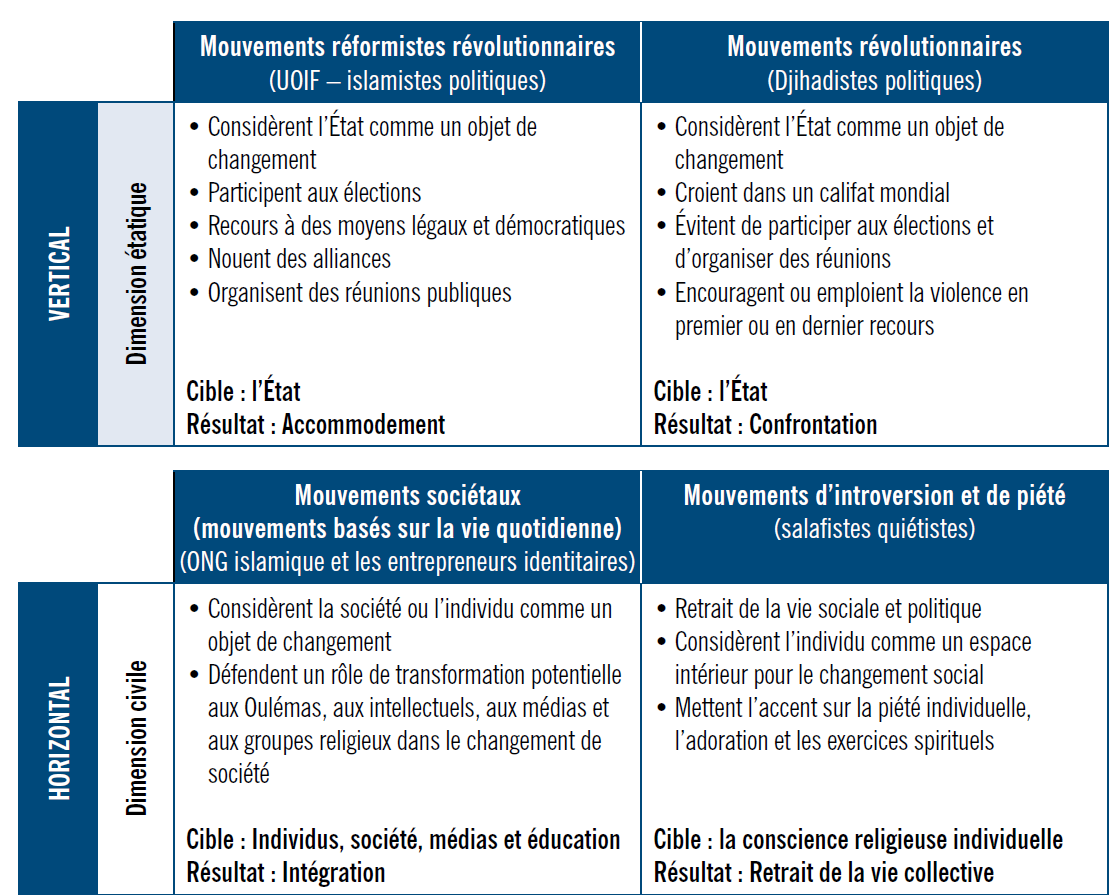
\includegraphics[width=\textwidth]{ImageIslamFrance/MouvementsIslamiques.png}

    \label{fig:mouvementsIslamiques}
\end{figure}

\paragraph{Différences entre les fondamentalismes frériste et
salafiste}

Si le salafisme est un islamisme, il convient de le distinguer de
l'islamisme politique tel que le promeuvent les Frères musulmans.
L'islam frériste est une idéologie moderne, produit de la rencontre
entre l'islam et la modernité occidentale, qui cherche, partout dans le
monde, à introduire l'islam dans la sphère politique. Les Frères
musulmans s'investissent donc dans la vie politique, en fondant des
partis politiques, en participant aux élections ou en militant en faveur
d'une islamisation du droit. Comme ils cherchent à intégrer l'islam dans
l'ensemble des sphères de la société, ils investissent aussi la sphère
politique, ainsi que le monde universitaire ou d'autres institutions.

Le salafisme, à l'inverse, cherche à « purifier » l'islam de l'influence
occidentale ainsi que des innovations et des évolutions qu'il a connues.
Il se fonde notamment sur un hadith, c'est-à-dire une citation de
Mahomet, selon lequel : \emph{« les meilleurs de ma communauté sont ceux
de ma génération, puis ceux qui les ont suivis, puis ceux qui leur ont
succédé ».} Le salafisme condamne à ce titre le chiisme, le soufisme,
mais aussi les autres rites sunnites non salafistes. Plus largement, le
salafisme condamne tout ce qui est postérieur à Mahomet ou toute chose
que le Prophète n'a pas admise. Par conséquent, la sécularisation,
l'État-nation, les partis politiques et tout ce qui relève la modernité
sont non-islamiques : les salafistes définissent l'islam comme
l'ensemble des pratiques, comportements et interprétations autorisée par
Mahomet.

Ainsi, si l'islamisme frériste et l'islamisme salafiste ont tous deux
pour objectif l'islamisation de la société et l'application de la
\emph{charia}, ils se distinguent par leurs méthodes. Les salafistes
prônent l'isolement et la séparation d'avec une société dans laquelle
ils ne se reconnaissent pas. Dans l'attente d'un départ vers un pays
musulman (la \emph{hijra}), où ils pourront se réaliser pleinement. Ils
créent un environnement dans lequel ils pourront vivre isolés du reste
de la société et qui leur permettra de concilier leur vie avec les
exigences de leur doctrine. À l'inverse, les fréristes n'adoptent pas
une stratégie de rupture mais d'intégration : seul l'investissement de
la sphère publique permettra de transformer la société, de la rendre
compatible avec les préceptes islamiques et d'imposer, à terme, la
\emph{charia}.




 

%----------------------------------------------------
\section{ L’avènement d’une génération de djihadistes français}

\mn{Cours 8 - Radicalisation Djihadisme (définitions, chiffres, rapports)} 
 
 \subsection{Chiffres des départs en Syrie/Irak depuis la France (pro-Daesh)}
1500 français sont allés rejoindre DAECH. Avec des lieux plus frappés que d'autres : 
\bi
\item Seine Saint Denis
\item Toulouse (78)
\item Trappe (70) 
\ei 
Hugo Micheron \sn{le Jihad français} explique Toulouse et Trappe par une maturation salafiste dans les années 90 et 2000 sur le terrain local en Toulouse et Trappe. Thèse de continuité au moins ideologique entre salafisme et jihadisme.

Un peu plus de 50\% vient de 15 départements seulement : grande banlieue populaire mais aussi des territoires plus inattendus : Vesoul ! Lunel ! Majoritairement des convertis, 6 de Vesoul par exemple. 

On a eu environ 500 détenus pour terrorisme dans les prisons en France et 300 revenants, qui sont revenus de DAECH. Il resterait 150 français dans les prisons syriennes et 15 en Irak. \sn{diverses sources, mentionnées par \CB}

AU niveau du Maghreb, 2000 maroccains sont allés en Syrie. Tunisie a eu le même nombre mais en nombre relatif, cela donne un des pays les plus touchés (après la tchétchénie).
 
\subsection{Définitions} 

\begin{Def}[Radicalisation]
« La radicalisation peut renvoyer à un ensemble de comportements ou de propos qualifiés d’extrême ou d’intransigeants et qui découlent d’une interprétation radicale des principes d’un système, qu’il soit de nature religieuse, politique ou économique. C’est en quelque sorte la première étape d’un engrenage irréversible qui \textit{peut} conduire à des passages à l’acte criminel et ultraviolent » \sn{Farhad Khosrokavar, Radicalisation, ed. FMSH, 2014}
\end{Def}

Une autre définition est donnée \sn{Romain Sèze, Xavier Crettiez, Bilel Aïnine, Saisir les mécanismes de la radicalisation violente : pour une analyse processuelle et biographique des engagements violents, Rapport pour la Mission de recherche Droit et Justice, INHESJ}:
\begin{Def}[Radicalisation]
« L’adoption progressive et évolutive d’une pensée rigide, vérité absolue et non négociable dont la logique structure la vision du monde des acteurs qui usent pour la faire entendre de répertoire d’actions violentes. »  

\end{Def}
Cette définition est reprise et développée dans : 
\begin{quote}
    « On définira donc la radicalisation comme l’adoption progressive et évolutive d’une pensée rigide, vérité absolue et non négociable, dont la logique structure la vision du monde des acteurs, qui usent pour la faire entendre de répertoires d’action violents, le plus souvent au sein de structures clandestines, formalisées ou virtuelles, qui les isolent des référents sociaux ordinaires et leur renvoient une projection grandiose d’eux-mêmes ». \sn{ Nicolas Lebourg et al., « Définir la radicalité pour mieux la combattre », \href{ttps://theconversation.com/}{The Conversation}, 15 avril 2018, h}
\end{quote}

\begin{Synthesis}
Les auteurs insistent ici sur la forme progressive et graduelle de la radicalisation. Influence du groupe, des organisations etc.
\end{Synthesis}

\paragraph{Biographie}
 Benjamin Chevallier et Cédric Passard, Publictionnaire, 6 avril 2018,  \url{http://publictionnaire.huma-num.fr/notice/radicalisation/}


\subsection{ Panorama sur les rapports}

\mn{lire les synthèses des rapports}

-Seze/Aïnine/Crettiez 2016, \href{http://www.gip-recherche-justice.fr/publication/saisir-les-mecanismes-de-la-radicalisation-violente-pour-une-analyse-processuelle-et-biographique-des-engagements-violents/ }{publication}

\mn{les les entretiens}

-Galland/Muxel 2017 (synthèse): \href{https://lejournal.cnrs.fr/nos-blogs/face-au-terrorisme-la-recherche-en-action/une-vaste-enquete-sur-la-radicalite-chez-les}{publication} 
Les collégiens et leur exposition au djihadisme. A fait parlé de lui.
-Hecker 2018: \href{https://www.ifri.org/fr/publications/etudes-de-lifri/focus-strategique/137-nuances-de-terrorisme-djihadistes-de-france-face}{publication}
-Bonelli/Carrié 2018:  \href{http://www.justice.gouv.fr/art_pix/Rapport_final_Bonelli_PJJ.PDF}{publication} 
-Sur la propagande djihadiste, voir le carnet de recherche d’Hasna Hussein; \href{https://cdradical.hypotheses.org/author/hussein}{Nature de la propagande jihadisme}. Noter la musique,... 

- Institut Montaigne : rapport en 2020 sur le profil des radicalisés. \href{https://www.institutmontaigne.org/publications/la-fabrique-de-lislamisme}{le rapport}. Intéressant panels de plusieurs milliers de personnes, avec données ouvertes et semi-ouvertes : données socio-culturelles,...

\subsection{Les différents modèles explicatifs de la radicalisation}
résumés très succinctement:
\paragraph{Olivier Roy - Paradigme Nihiliste de la radicalisation}
nihilisme, sécularisés, et velléités d’actions, d’aventures, d’héroïsme, voir de suicide déguisé en acte héroïque.  Important : phénomène de « déculturation » et même « d’exculturation ».\sn{-Olivier Roy \textit{Le djihad et la mort}, 2015.}
 Les jeunes ont des profils sécularisés, à la recherche d'aventure. N'exclut pas les facteurs religieux. Peu intégrés et peu religieux.

\paragraph{Gilles Képel, Bernard Rougier - Paradigme idéologico-religieux de la radicalisation}
le poids de l’idéologie religieuse salafiste et djihadiste \sn{-Gilles Képel, Bernard Rougier (Terreur sur l’Hexagone, 2016), \textit{les territoires conquis de l'Islamisme}, en prison}, des conceptions islamistes belliqueuses. Gilles Képel n'exclut pas la question sociale comme terreau du départ. 


\paragraph{Alain Bertho (paradigme "social")}, et une partie importante des sociologues de la pauvreté, de la précarité et des marges urbaines: « Islamisation de la radicalité » (Les enfants du chaos, 2016). Une partie des sociologues partage cette analysation .

\paragraph{François Burgat (paradigme "politique et géopolitique")} les régimes politiques autoritaires, la géopolitique, et la stigmatisation comme cause principale de la communauté musulmane en France... On pourrait opposer l'exemple du Maroc avec 2000 jeunes et le même nombre en Tunisie. 

\paragraph{Fethi Benslama (paradigme "psy")}  détresse psychique, pb familiaux, ruptures, absence du père etc. + également rôle du gourou, donc radicalisation comprise comme le résultat d’une manipulation mentale. Phénomène sectaire. Donia Bouzara. Il n'exclut pas le facteur religieux comme facteur explicatif : "volonté d'être sur-musulman".

\begin{Synthesis}
On peut aussi regarder les différentes populations et appliquer les différents paradigmes plus ou moins pertinents sur telle ou telle population.
\end{Synthesis}


\paragraph{Quels sont les facteurs de radicalisation ?}
\mn{Rapport Montaigne}


Au-delà de la situation {géopolitique (en Syrie, en Palestine, en
Irak ou ailleurs), la quête d'identité,} notamment des jeunes nés en
Occident, apparaît comme l'un des facteurs explicatifs majeurs. Beaucoup
d'entre eux, ont le sentiment d'être, certes des citoyens aux yeux de la
loi, mais privés de toute reconnaissance culturelle ou sociale.

Les prédicateurs radicaux développent l'idée dualiste apocalyptique de «
guerre sainte », entre leurs fidèles alliés et leurs ennemis impies.
{Le « nous » contre le} « eux ».


Cette situation s'est accrue pour les deuxième et troisième générations
d'immigrés, en raison de deux principaux phénomènes :


\begin{itemize}
\item
  
  \textbf{le manque de sentiment d'appartenance au pays d'origine des
  parents,} qui s'approfondit en raison de plusieurs expériences de
  discrimination vécues des deux côtés \emph{(« Je ne suis pas Français,
  je ne suis pas blédard. Que suis-je ? Je suis musulman »)} ;
  
\item ~
  le manque d'opportunités socio-économiques.
\end{itemize}

\paragraph{Quel est le lien entre internet et la radicalisation ? Une
  propagande huilée}



Internet est le l{ieu idéal de radicalisation et de galvanisation
collective,} puisque cet outil permet -- de manière plus ou moins
sécurisée et anonyme -- de s'informer et d'entrer en contact avec des
mouvements djihadistes. En outre, les barrières géographiques n'étant
plus une limite, échanger avec des radicaux du monde entier est
désormais possible.

Lors de ces échanges :


\begin{itemize}
\item
  
  l'accent est mis sur {\emph{« l'empowerment »} et l'aspect
  égalitaire des groupes djihadistes :} chacun a sa chance, chacun peut
  accomplir de « grandes choses » ;
  
\item
  
  l'individu djihadiste aura, en conséquence, la possibilité de devenir
  un héros, sa propre mort lui ouvre les portes du paradis et de la
  gloire ;
  
\item
  
  pour les femmes, l'accent est mis sur la vertu et sur la participation
  à une {action humanitaire} afin de sauver la veuve, l'orphelin
  et un peuple martyrisé par ses dirigeants et par ses alliés impies ou
  apostats.
  
\end{itemize}


L'islamisme radical utilise donc internet afin d'inculquer :


\begin{itemize}
\item
  une certaine interprétation de la religion ;
\item
  la culture du sacrifice, du martyre ;
\item
  la nécessité de choisir un camp (l'« Occident » ou la voie sacrée de
  l'islam) ;
\end{itemize}

\paragraph{Quel est le lien entre salafisation et terrorisme ?}
\subparagraph{Étape 1 :
l'endoctrinement}


L'endoctrinement, l'intensification des croyances et l'adoption complète
du mode
de vie salafiste créent en partie les conditions qui invitent à soutenir
le djihad.

Le processus d'endoctrinement est dirigé par un {censeur
spirituel.} Cette phase est ainsi marquée par des rencontres avec des
individus partageant les mêmes croyances, qui aident à approfondir la
doctrine et l'engagement. Les pairs deviennent fondamentaux afin de
soutenir le processus de radicalisation.

Le moment clé de ce processus est l'acceptation de l'idéologie
politico-religieuse, qui légitime l'utilisation de la violence envers
les non musulmans.


\subparagraph{Étape 2 : le basculement}


Deux indicateurs de basculement sont particulièrement importants.


\begin{enumerate}
\def\labelenumi{\arabic{enumi}.}
\item
  \textbf{L'abandon de la mosquée.} La mosquée n'est plus fréquentée par
  les individus radicalisés. Elle est perçue comme un environnement à
  risque et l'abandon de cet espace est souvent accompagné d'une dispute
  avec d'autres membres de la mosquée. La mosquée est perçue comme une
  menace, parce qu'elle est souvent surveillée par les services de
  renseignement.
\item
  \textbf{La politisation des nouvelles croyances.} Les radicalisés
  commencent à transférer leurs croyances dans la vie quotidienne. Les
  événements internationaux sont interprétés à partir de cette nouvelle
  vision souvent dichotomique (« nous » contre « eux », les non
  musulmans contre les musulmans).
\end{enumerate}





\subparagraph{Étape 3 : la djihadisation}


Il s'agit du moment où les personnes s'auto-identifient à des guerriers
sacrés \emph{(« moudjahidine »)} et perçoivent le \emph{djihad} comme un
devoir. Cela correspond à une phase de planification durant laquelle le
groupe solidifie ses liens et se consolide. L'individu radicalisé peut
alors parcourir les étapes suivantes :


\begin{itemize}
\item
  
  accepter le djihad, et potentiellement se rendre dans un camp
  d'entraînement ;
  
\item
  
  entraînement physique et mental ;
  
\item
  
  planification d'une attaque ;
  
\item
  
  passage à l'acte.
  
\end{itemize}


  \paragraph{Quels sont les obstacles à la radicalisation ?}



Pour être considérés \textbf{résistants à l'extrémisme violent,} les
individus en question doivent avoir déjà été exposés à des idéologies
radicales ou même avoir déjà flirté avec une mentalité radicale, mais
avoir finalement rejeté la violence.

Il existe quatre principaux facteurs de résistance à la radicalisation :


\begin{itemize}
\item
  
  \textbf{la répugnance morale,} c'est-à-dire un désaccord profond avec
  l'idée de faire usage de la violence pour parvenir à ses fins ou pour
  occasionner des changements sociaux, politiques, économiques ou
  religieux ;
  
\item
  
  \textbf{l'impression d'inefficacité de la violence.} Cette impression
  peut être occasionnée soit par de l'apathie, c'est-à-dire parce que
  ces individus n'ont aucun désir de provoquer du changement ou n'en
  éprouvent pas le besoin, ou parce qu'ils ont emprunté des chemins
  alternatifs non violents pour provoquer ces changements ;
  
\item
  
  \textbf{les coûts perçus,} qui peuvent être :
  


\begin{itemize}
\item
  des coûts logistiques ;
\item
  des coûts financiers ;
\item
  des obligations familiales ;
\item
  ou la peur de la répression ;
 \end{itemize}

  \item
    
    l'absence de liens sociaux qui encouragent ou renforcent le
    processus de radicalisation.
    
 
\end{itemize}




%----------------------------------------------------
\section{A parallel society is developing in parts of Muslim Britain}

\marginnote{
As a new book by Ed Husain explains
Britain
Jun 5th 2021} 

Ed Husain’s new book, “Among the Mosques”, is a fascinating addition to this tradition, taking readers inside religious institutions that most non-Muslims only experience as domes on the horizon. The country’s first two mosques were founded in Liverpool in 1887, in a terraced house, and in Woking in 1889, on a grander scale. There are now almost 2,000 serving a Muslim population of more than 3m. Some heavily Muslim areas such as Blackburn’s Bastwell district have several in the same street. But what goes on inside? And what is their relationship with wider society?

Mr Husain is the ideal man to answer these questions. The son of an Indian father and a mother who migrated from what is today Bangladesh, he won a prize for reciting the Koran as a child and spent much of his 20s in the Middle East perfecting his Arabic. He has written two books on Islam and has a broad intellectual hinterland. He wrote a phd thesis under the supervision of the conservative British philosopher, Roger Scruton, and has worked for a number of think-tanks including the Council on Foreign Relations in America.


Mr Husain discovered much to be pleased about. Britain has absorbed a big Muslim population better than its ancient foe, France. On May 6th London re-elected its first Muslim mayor, Labour’s Sadiq Khan. Several young politicians such as Naz Shah, mp for Bradford West, represent the modern face of the religion.

There is also a darker story. The British establishment that presided over the immigration which followed the second world war expected Islamic migrants to melt into wider society and relax their religious views. But in parts of the country Muslim communities are distancing themselves from wider British society and adopting stricter versions of their faith.

This is particularly true in the old mill towns of Yorkshire and Lancashire, which now contain parallel societies, where the faithful can live their day-to-day lives without mixing. Mosques run schools and pronounce on Islamic law. Restaurants offer gender segregation under the polite name of “family seating”.

These societies are dominated by a clerical class that extends its influence into secular society by, for example, endorsing candidates for Parliament. Mr Husain visited mosque after mosque that taught a highly literal interpretation of Islam, sometimes clinging to arguments that are being dropped in the Middle East. He saw shops displaying books that advocate stoning gays or keeping wives in purdah or waging jihad. Sayyid Qutb (p.\pageref{theol:SayyidQutb}), Osama bin Laden’s favourite philosopher, appeared often.

Many of these clerics belong to religious groupings with roots far from these shores. Saudi Wahhabis pour money into British mosques and offer all-expenses-paid scholarships to young British Muslims. More surprising is the importance of the Deobandis \sn{Le deobandi ou deobandisme est une école de pensée musulmane sunnite, très présente en Asie du Sud (Pakistan, Inde et Afghanistan). Apparue dans les Indes britanniques en 1867 en réaction à la colonisation, elle tire son nom de la ville de Deoband, dans l'État de l'Uttar Pradesh dans le nord de l'Inde, qui a vu naître sa première école1. Se réclamant de Abu Hanifa, juriste musulman du viiie siècle fondateur de l'école hanafite, elle prône un islam traditionaliste et apolitique ainsi qu'une lecture littéraliste des textes.L'école deobandi a aussi bien été l'une des sources de pensée des talibans afghans que du Tablighi Jamaat. Le nombre d'étudiants inscrits au Pakistan dans des madrasas déobandi serait en croissance rapide (multiplication par deux en 2007). Cette école est souvent en conflit avec l'école barelvie, également très présente en Asie du Sud.}. 

Mr Husain claims more than half of the country’s mosques now belong to the movement, which began in India and seeks to rebuild the caliphate from the ground up, convert by convert. Dewsbury, a historic market town in Yorkshire, is the European capital of the largest Muslim organisation in the world, the Tableeghi Jamaat, the movement’s evangelical arm.

Why does this matter? Religious minorities have always clung together, the better to preserve their faith. Look at the Quakers during the Industrial Revolution or Orthodox Jews in Manchester or London today. Isn’t “a parallel society” just a derogatory name for a flourishing subculture? And isn’t the Catholic church also an example of foreign influence? It is no business of the state to make windows into people’s souls.

There are nevertheless good reasons to be worried. One is the paradox of toleration. There are limits to how much liberal societies can tolerate people who call for gays to be stoned or who denounce Ms Shah as “a dog” because she fails to wear a hijab. The radicalised version of Islam being preached by clerics not only promotes intolerance but also fosters extremism.

A second is the paradox of diversity. The welfare state that liberals hold dear depends for its legitimacy on people feeling that they have a common identity. Robert Putnam, a Harvard sociologist, has demonstrated that support for the provision of public goods falls sharply if people think that the recipients are strikingly different from them. It is hard to be more strikingly different than the parallel communities of Dewsbury and Bradford.
\subsection{State failure}
The third is more practical. Britain is witnessing a struggle for the soul of Islam. But the state has repeatedly acted as if it is on the side of the forces of reaction rather than those of enlightenment. It has kowtowed to self-proclaimed community leaders, mistaking hardline beliefs for “authenticity”. It has tolerated schools such as Darul Uloom, in Rochdale, that combines gcse instruction with requiring students to memorise the Hadiths, including ones about beating wives and stoning homosexuals. And it has failed to make a compelling case for Britishness. Mr Husain points out that many Muslim children get a warts-and-all account of British history from their schools, while hearing constant praise for Turkey and Saudi Arabia in their madrassas. The trauma of Brexit has created a palpable desire to cure many of the social and geographic divisions that threaten to divide the country into warring tribes. Mr Husain makes a compelling case that that quest should not ignore the world of the mosque. 
% --------------------------------------------------
\section{Pour aller plus loin}
-Bibliographie de la partie :
AMGHAR, Samir, Le salafisme d’aujourd’hui. Mouvements sectaires en Occident,
Michalon, 2011.
CARRE Olivier, SEURAT Michel, Les Frères Musulmans (1928-1982), L'Harmattan,
2001 (1983)
MICHERON Hugo, Le jihadisme français. Quartiers, Syrie, Prisons, Gallimard, 2020.



% --------------------------------------------------


\section{Faudra-t-il sauver les salafistes ?}

\mn{La Croix, le 26/01/2021 à 13:25 Modifié le 26/01/2021 à 13:28}
\textit{Olivier Hanne, médiéviste (université de Poitiers), chercheur en islamologie, explique que les courants salafistes prônent un islam épuré et intégriste mais qu’ils rejettent le recours à la violence. }
Le gouvernement français a voulu lancer en octobre 2019 une offensive
contre l'islamisme et les courants radicaux, rapidement relayée par un
emballement médiatique qui a échappé à tout contrôle. Or, l'ennemi
désigné n'a nullement été identifié selon des termes juridiques, pas
plus que ses torts. On lui reproche sa piété rigoureuse, son voile, sa
pratique du jeûne de Ramadan, sa barbe fournie, son refus de toucher les
femmes, ce qui le rapproche dangereusement de n'importe quel fidèle
conservateur.

L'offensive vise donc une manière de concevoir la piété musulmane, et
nullement une qualification criminelle ou une atteinte à l'ordre public.
C'est dire que nous sommes confrontés à un « délit de sale gueule »,
lequel échappe à la tradition juridique républicaine, délit qui est
indiscernable, sans limite, extensible, mais politiquement pratique
auprès d'une opinion chauffée à blanc par les attentats et
l'immigration.

\subsection{Un engagement d'abord religieux}

Si l'islamiste ainsi décrit ressemble évidemment
au~\href{https://www.la-croix.com/Religion/Islam/Quest-salafisme-2018-10-14-1200975866}{\underline{salafiste}},
c'est oublier un peu vite que l'écrasante majorité des~\emph{salafi~}--
ceux qui sont attachés au modèle des « anciens » (les~\emph{salaf}),
c'est-à-dire les compagnons du Prophète -- se veulent quiétistes : leur
mode d'action est la prédication et l'action missionnaire
(la~\emph{da`wa}). Le salafiste souhaite d'abord vivre un islam épuré et
intégriste -- au sens d'intégral -- dans le cadre de sa famille et de sa
communauté.

Ce mouvement est distinct d'un engagement politique, de sorte que les
salafistes sont rarement liés aux Frères musulmans, qui eux forment un
mouvement politique. Si la matrice religieuse et idéologique du
salafisme imprègne les mentalités djihadistes, elle ne se confond pas
avec celles-ci, ni dans la pensée, ni dans les faits. La radicalisation
concerne donc à des degrés différents et sous des formes incomparables
les sympathisants du salafisme et les partisans du djihadisme de Daech.
Les premiers ont un engagement d'abord religieux, tandis que les autres
sont mus à la fois par la volonté de puissance, des facteurs politiques,
sociaux et religieux.

\subsection{L'autodidacte de l'islam présente plus de risques que le
salafiste}

L'hostilité des salafistes envers les courants djihadistes a été prouvée
à de nombreuses reprises par des déclarations publiques et surtout en
fournissant du renseignement de qualité auprès des services de police.
Le meilleur ennemi du terroriste est souvent le~\emph{salafi}, et
l'autodidacte de l'islam présente plus de risques que le salafiste.

En outre, le salafisme n'a pas été désavoué par les représentants du
culte musulman pour la simple raison que ce courant n'est pas une
idéologie : il faudrait donc lui enlever son~\emph{isme}~final et
l'appeler, selon la tradition religieuse, la~\emph{salafiya~}; il s'agit
d'un vieux courant légitime de l'islam, qui a fourni des générations
d'imams et de lettrés attachés au sens littéral du Coran et de la Sunna.

\subsection{Un « écosystème » étroit mais rassurant}

Il est évident que le salafisme représente une alternative culturelle et
sociale au modèle français, modèle égalitaire, inclusif, ouvert (au
moins en théorie). Les quelques salafi que j'ai connus -- des convertis
à 25 ou 30 \% d'entre eux -- vivaient dans un étroit triangle
géographique. Parce qu'ils souhaitent faire les cinq prières à leur
heure, sans les décaler, et ce dans une salle de prière, ils sont
contraints de vivre et de travailler non loin d'une mosquée. Ils passent
ainsi de leur habitation au lieu de travail et à la salle de prière,
lesquels se situent nécessairement dans un « écosystème » étroit mais
rassurant. Ils ne peuvent guère être exigeants sur le plan
professionnel.



Le salafisme, qui représente au moins 40 000 individus, est socialement
dangereux car il impose l'auto-ségrégation, le refus des contacts avec «
ceux qui n'en sont pas ». C'est la raison pour laquelle les spécialistes
des questions de sécurité se refusent à les impliquer dans la lutte
contre le djihadisme. Salafistes et terroristes participeraient à une
même matrice intellectuelle, celle du bien contre le mal, une sorte de
vision sectaire du monde. La différence vient du rapport à la violence :
assumé chez les djihadistes, rejeté chez les salafistes. Leur
fondamentalisme présente l'avantage d'une certaine forme de morale : à
Sartrouville les quartiers salafisés ont vu s'effondrer la toxicomanie
et la délinquance, avec le soutien de la mairie.

\subsection{Confondre l'approche culturelle avec la lutte contre le
terrorisme}

Ces courants ne peuvent être incriminés sur le plan sécuritaire. On
confond donc l'approche culturelle avec la lutte contre le terrorisme. À
moins de changer tout le droit européen, la première doit être menée par
l'éducation, la philosophie, la raison, le débat ; quant à la seconde
elle doit s'appuyer sur le droit et sur des qualifications pénales, et
non sur de vagues impressions de « radicalisation », notion qui n'a
toujours pas été appréhendée de façon rigoureuse en termes sociologiques
et psychologiques.

Comme la guerre d'Algérie nous l'enseigne, une telle manière de
concevoir l'action politique va aboutir à l'effet inverse de celui
recherché : le renforcement de la méfiance collective, le repli
communautaire du côté musulman, l'action violente du côté des « anti »,
et, finalement, la fragmentation sociale et l'insécurité.

\section{Islam : les fumées de la radicalisation}
\mn{La Croix le 27/01/2021 à 13:08}
\textit{Olivier Hanne, médiéviste (université de Poitiers), chercheur en
islamologie, estime qu'il est très difficile de définir le parcours type
d'une personne radicalisée.}
 

Qui parle d'islam aujourd'hui pense aussitôt à la radicalisation. En
2015, on estimait entre 8 000 et 10 000 le nombre de Français
radicalisés. Leurs profils sont si variés qu'il est difficile de donner
des catégories fixes : les mineurs représentent 25 \% des cas, les
femmes 27 \%, les personnes signalées sont plutôt jeunes (entre 16 et 30
ans), leur niveau scolaire est généralement faible, même si l'on
rencontre des diplômés.

La plupart travaillent. Internet représente pour tous ces individus un
passage obligé, même s'il se concrétise différemment : terrain initial
de la radicalisation, facteur de renforcement ou vecteur unique de
l'expression radicale, le partage des contenus djihadistes sur Internet
n'a pas du tout la même fonction chez une adolescente connectée, un
salafiste convaincu et un combattant expérimenté déjà parti en Syrie.

\subsection{Les autorités font feu de tout bois}

De toute évidence, l'attraction pour la radicalité religieuse n'est pas
nécessairement liée à un phénomène de rupture sociale. Les failles de la
société contemporaine (éclatement des familles, déclin des autorités et
des idéologies, chômage, ghettoïsation) créent un terreau facilitateur,
mais nullement déterminant. La frustration individuelle alimente le
recours à des convictions extrêmes, voire le passage à l'acte
terroriste, mais n'est qu'un facteur parmi tant d'autres.

Les autorités font feu de tout bois pour tenter de faire face à une
radicalisation multiforme. En avril 2015, le premier ministre français,
Manuel Valls, annonçait l'ouverture d'une dizaine de centres de
prévention de la radicalisation, dont la plupart furent un échec. Des
sites Internet officiels sont créés et proposent des fiches techniques
contre la radicalisation et le terrorisme, dont le contenu est souvent
simple, voire binaire. Ainsi sur le site
français~\emph{stop-djihadisme.gouv.fr}, un bandeau intitulé «
Radicalisation djihadiste, les premiers signes qui peuvent alerter »
énonce pêle-mêle : « ils se méfient des anciens amis qu'ils considèrent
maintenant comme des impurs » ; « ils changent brutalement leurs
habitudes alimentaires » ; « ils arrêtent d'écouter de la musique car
elle les détourne de leur mission » ; « ils ne regardent plus la
télévision et ne vont plus au cinéma ». Autant de signes extérieurs qui
se rapprochent de l'adolescente anorexique\ldots{} L'efficacité de ces
dispositifs a d'ailleurs été très contestée dès 2015.

\subsection{L'État, tenté d'être omniprésent}

Toute l'entreprise de déradicalisation définit en creux le modèle
positif occidental : monde de loisirs, de consommation, d'épanouissement
personnel et professionnel. Le vocabulaire de la radicalisation masque
le rejet de ce modèle culturel. Et les pouvoirs publics d'hésiter à
appeler leur objectif par son vrai nom : le reconditionnement mental.

Le danger de la déradicalisation se situe dans l'élargissement des
intrusions de l'État : en voulant réinsérer, l'État pénètre dans
l'intimité des individus afin de redéfinir le religieux et lui redonner
une place acceptable. Or, l'État a-t-il compétence pour définir ce
qu'est l'islam, le « bon » islam ? Ne sachant cerner la menace, l'État
est tenté d'être omniprésent, sans en avoir la capacité légale. La
déradicalisation pourrait relever de la posture intellectuelle.

Le problème vient sans doute des hésitations du vocabulaire. Car,
après-tout, qu'est-ce que la radicalisation ? Au
XIX\textsuperscript{e}~le mot anglais~\emph{radical}~était employé pour
désigner les partis politiques britanniques exigeant une réforme
démocratique libérale. Transféré tel quel en France, on l'appliqua aux
partis de gauche, laïques et libéraux qui voulaient réformer la société.

\subsection{Réactions épidermiques}

Le verbe « radicaliser » fut employé régulièrement dans les années
1960-1970 dans une acception politique avec l'idée de « devenir plus
intransigeant, se durcir » ou « plus extrême ». Le premier sens était
donc politique et pas nécessairement négatif. Se déradicaliser était un
synonyme pour « se compromettre ». Appliqué à l'islamisme, le verbe
impose une redéfinition complète des termes : à partir de quand
juge-t-on l'islam intransigeant ou extrême ? par rapport à quelle norme
? à quelle moyenne ?

Les réactions épidermiques qui ont suivi le meurtre de l'enseignant de
Conflans-Sainte-Honorine en octobre 2020 sont tristement révélatrices :
les imams doivent s'exprimer ! les musulmans doivent désavouer le
terrorisme et faire allégeance à la France ! Mais quand ils le font,
c'est encore insuffisant, déloyal et mensonger. Le gouvernement proposa
même qu'ils prient pour la République au cours de la prière collective
du vendredi. Nos références sur la question religieuse restent
tragiquement celles de la Révolution française : comme il y eut les «
prêtres jureurs », adhérant à la loi, contre les « prêtres réfractaires
», obstinés dans leur obéissance à Rome, de la même façon il nous faut
des « imams jureurs », intimement républicains. L'État se retrouve donc
juge des reins et des cœurs.

